\def\sevenSegWidth{2.25}
\def\sevenSegHeight{3}

\ctikzsubcircuitdef{spicSevenSeg} {
    north, south, east, west,
    northeast, northwest, southeast, southwest,
    center,
    pin-01, pin-02, pin-03, pin-04, pin-05,
    pin-06, pin-07, pin-08, pin-09, pin-10%
} {
    coordinate (#1-origin)
    ++(1.125,-1.5)
    node [inner sep = 0pt, anchor = center] {
        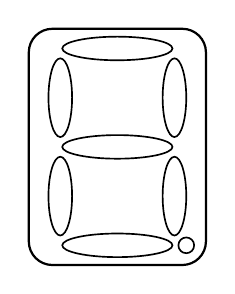
\begin{tikzpicture}
            \draw [rounded corners = 3mm, thick]
            (0,0) rectangle (\sevenSegWidth,-\sevenSegHeight)
            (0,0) coordinate (segorigin)
            ;
            %% horizontal segments
            \draw [semithick]
            (segorigin) ++(1.125,-0.25)
            ellipse [x radius = 0.7, y radius = 0.15]
            ;
            \draw [semithick]
            (segorigin) ++(0,-\sevenSegHeight) ++(1.125,0.25)
            ellipse [x radius = 0.7, y radius = 0.15]
            ;
            \draw [semithick]
            (segorigin) ++(1.125,-1.5)
            ellipse [x radius = 0.7, y radius = 0.15]
            ;
            %% vertical segments
            \draw [semithick]
            (segorigin) ++(0,-0.125) ++(0.4,-0.75)
            ellipse [x radius = 0.15, y radius = 0.5]
            ;
            \draw [semithick]
            (segorigin) ++(\sevenSegWidth,0) ++(0,-0.125) ++(-0.4,-0.75)
            ellipse [x radius = 0.15, y radius = 0.5]
            ;
            \draw [semithick]
            (segorigin) ++(0,-1.5) ++(0,0.125) ++(0.4,-0.75)
            ellipse [x radius = 0.15, y radius = 0.5]
            ;
            \draw [semithick]
            (segorigin) ++(0,-1.5) ++(\sevenSegWidth,0) ++(0,0.125) ++(-0.4,-0.75)
            ellipse [x radius = 0.15, y radius = 0.5]
            ;
            %% ...dot
            \draw [semithick]
            (\sevenSegWidth,-\sevenSegHeight)
            ++(-0.25,0.25)
            circle (0.1)
            ;
        \end{tikzpicture}
    }
    %% top pins
    (#1-origin) ++(1.125,0.25)
    coordinate (#1-pin-08)
    %%
    (#1-origin) ++(1.125,0.25)
    ++(0.4,0) coordinate (#1-pin-07)
    ++(0.4,0) coordinate (#1-pin-06)
    %%
    (#1-origin) ++(1.125,0.25)
    ++(-0.4,0) coordinate (#1-pin-09)
    ++(-0.4,0) coordinate (#1-pin-10)
    %% bottom pins
    (#1-origin) ++(0,-\sevenSegHeight)
    coordinate (#1-bottom)
    (#1-bottom) ++(1.125,-0.25)
    coordinate (#1-pin-03)
    %%
    (#1-bottom) ++(1.125,-0.25)
    ++(0.4,0) coordinate (#1-pin-04)
    ++(0.4,0) coordinate (#1-pin-05)
    %%
    (#1-bottom) ++(1.125,-0.25)
    ++(-0.4,0) coordinate (#1-pin-02)
    ++(-0.4,0) coordinate (#1-pin-01)
    \markgeocoordinate {#1}
    {(#1-pin-10)} {(#1-pin-01)}
    {(#1-origin)} {(#1-origin) ++(\sevenSegWidth,-\sevenSegHeight)}
}

\ctikzsubcircuitactivate{spicSevenSeg}

\newcommand\ovrSevenSegPinHoles[1] {
    (#1-pin-01) node [ocirc] {}
    (#1-pin-02) node [ocirc] {}
    (#1-pin-03) node [ocirc] {}
    (#1-pin-04) node [ocirc] {}
    (#1-pin-05) node [ocirc] {}
    (#1-pin-06) node [ocirc] {}
    (#1-pin-07) node [ocirc] {}
    (#1-pin-08) node [ocirc] {}
    (#1-pin-09) node [ocirc] {}
    (#1-pin-10) node [ocirc] {}
}

\newcommand\ovrSevenSegCathodePinHoles[1] {
    (#1-pin-01) node [ocirc] {}
    (#1-pin-02) node [ocirc] {}
    (#1-pin-04) node [ocirc] {}
    (#1-pin-05) node [ocirc] {}
    (#1-pin-06) node [ocirc] {}
    (#1-pin-07) node [ocirc] {}
    (#1-pin-09) node [ocirc] {}
    (#1-pin-10) node [ocirc] {}
}
